\chapter{Математические предварительные сведения}
\label{chap:preliminaries}

\begin{supportbox}{Об этой главе}
Здесь мы сжато излагаем математические концепции, необходимые для понимания книги. Мы предполагаем наличие предварительных знаний по всем этим темам, сосредотачиваясь больше на описании специфической нотации и предоставлении целостного обзора. По возможности мы подчеркиваем связь между некоторым из этого материала (например, тензорами) и их практической реализацией.
\end{supportbox}

Глава состоит из трех частей, последовательно вытекающих друг из друга: начиная с \textbf{линейной алгебры}, переходя к определению \textbf{градиентов} для $n$-мерных объектов и, наконец, к тому, как мы можем \textbf{оптимизировать} функции, используя эти градиенты. Самостоятельный обзор \textbf{теории вероятностей} представлен в Приложении \ref{chap:probability_theory}, с акцентом на принцип \textbf{максимального правдоподобия}. Эта глава насыщена содержанием и определениями: потерпите меня немного!


\section{Линейная алгебра}
\label{sec:linear_algebra}

Здесь мы напомним некоторые основные концепции из линейной алгебры, которые будут полезны в дальнейшем (и для согласования общей нотации). Большая часть книги вращается вокруг идеи \textbf{тензора}.

\begin{definition}[Тензоры] \addbottle
  \textbf{Тензор} $X$ — это $n$-мерный массив элементов одного и того же типа. Мы используем $X \sim (s_1, s_2, \ldots, s_n)$ для краткого обозначения \textbf{формы} тензора.
\end{definition}
%
При $n=0$ мы получаем \textbf{скаляры} (одиночные значения), при $n=1$ — \textbf{векторы}, при $n=2$ — \textbf{матрицы}, а в остальных случаях — многомерные массивы. Напомним, что мы используем строчную букву $x$ для скаляров, строчную жирную $\mathbf{x}$ для векторов и прописную жирную $\mathbf{X}$ для матриц. Тензоры в описанном здесь смысле являются фундаментальными в глубоком обучении, поскольку они хорошо подходят для массово-параллельной реализации, например, с использованием GPU или более специализированного оборудования (например, TPU, IPU).

Тензор описывается типом его элементов и его \textit{формой}. Большая часть нашего обсуждения будет сосредоточена на тензорах со значениями с плавающей запятой (конкретный формат которых мы рассмотрим позже), но они также могут быть определены для целых чисел (например, в классификации) или для строк (например, для текста). Тензоры можно \textbf{индексировать} для получения \textbf{срезов} (подмножеств) их значений, и здесь применяются большинство соглашений из индексации NumPy\footnote{См. обзор на \url{https://numpy.org/doc/stable/user/basics.indexing.html}. Для удобочитаемости в книге мы индексируем с $1$, а не с $0$.}. Для простых уравнений мы используем нижние индексы: например, для 3-мерного тензора $X \sim (a, b, c)$ мы можем написать $X_i$ для обозначения среза размером $(b,c)$ или $X_{ijk}$ для одного скаляра. Мы используем запятые для более сложных выражений, таких как $X_{i, :, j:k}$ для обозначения среза размером $(b, k-j)$. Когда необходимо избежать загромождения, мы используем светло-серую нотацию:

\begin{equation*}
    \idx{X}{ijk}
\end{equation*}
%
чтобы визуально отделить часть с индексацией от остального, где аргумент $\idx{\bullet}{}$ также может быть выражением.

\subsection{Основные операции с векторами}
\label{subsec:common_vector_operations}

Мы в основном занимаемся моделями, которые можно записать как композицию дифференцируемых операций. Фактически, большинство наших моделей будут состоять из базовых композиций сумм, умножений и некоторых дополнительных нелинейностей, таких как экспонента $\exp(x)$, синусы и косинусы, и квадратные корни.

Векторы $\mathbf{x} \sim (d)$ являются примерами 1-мерных тензоров. В книгах по линейной алгебре уделяется внимание различению векторов-столбцов $\mathbf{x}$ и векторов-строк $\mathbf{x}^\top$, и мы постараемся придерживаться этого соглашения как можно точнее. В коде это сложнее, потому что векторы-строки и векторы-столбцы соответствуют 2-мерным тензорам формы $(1,d)$ или $(d,1)$, которые отличаются от 1-мерных тензоров формы $(d)$. Это важно помнить, потому что большинство фреймворков реализуют правила трансляции (broadcasting)\footnote{См.: \url{https://numpy.org/doc/stable/user/basics.broadcasting.html}. Вкратце, трансляция выравнивает формы тензоров справа и повторяет тензор, когда это возможно, чтобы согласовать две формы.} вдохновленные NumPy, что приводит к неинтуитивному поведению. См. Листинг \ref{code:broadcasting} для примера очень распространенной ошибки, возникающей при неявной трансляции форм тензоров.

\begin{mypy}{Пример (вероятно, некорректной) трансляции, приводящей к матричному выводу из поэлементной операции над двумя векторами из-за их форм. Тот же результат можно получить практически в любом фреймворке (NumPy, TensorFlow, JAX, ...).}{code:broadcasting}
import torch
x = torch.randn((4, 1))  # Вектор-"столбец"
y = torch.randn((4,))    # 1-мерный тензор
print((x + y).shape)        
# [Out]: (4,4) (из-за трансляции!)
\end{mypy}

Векторы обладают собственной алгеброй (которую мы называем \textbf{векторным пространством}), в том смысле, что любые два вектора $\mathbf{x}$ и $\mathbf{y}$ одинаковой формы могут быть линейно скомбинированы $\mathbf{z} = a\mathbf{x} + b\mathbf{y}$ для получения третьего вектора:
%
$$
z_i=ax_i+by_i
$$
%
Если мы понимаем вектор как точку в $d$-мерном евклидовом пространстве, сумма интерпретируется как построение параллелограмма, а расстояние вектора от начала координат задается евклидовой ($\ell_2$) нормой:
%
$$
\lVert \mathbf{x} \rVert=\sqrt{\sum_i x_i^2}
$$
%
Квадрат нормы $\lVert \mathbf{x} \rVert^2$ представляет особый интерес, поскольку он соответствует сумме квадратов элементов. Основная векторная операция, которая нас интересует, — это \textbf{скалярное произведение}, которое получается путем поэлементного умножения двух векторов и суммирования полученных значений.


\begin{definition}[Скалярное произведение]   \addbottle
    Скалярное произведение двух векторов $\mathbf{x}, \mathbf{y} \sim (d)$ задается как:
    \begin{equation}
            \langle \mathbf{x},\mathbf{y}\rangle=\mathbf{x}^\top\mathbf{y}=\sum_ix_iy_i
    \end{equation}
\end{definition}
%
Обозначение $\langle \bullet, \bullet \rangle$ распространено в физике, и мы иногда используем его для ясности. Важно отметить, что скалярное произведение двух векторов является скаляром. Например, если $\mathbf{x} = [0.1, 0, -0.3]$ и $\mathbf{y}=[-4.0, 0.05, 0.1]$:
%
\begin{equation*}
    \langle \mathbf{x}, \mathbf{y} \rangle = - 0.4 + 0 - 0.03 = - 0.43
\end{equation*}
%
Простая геометрическая интерпретация скалярного произведения дается его связью с углом $\alpha$ между двумя векторами:
%
\begin{equation}
    \mathbf{x}^\top\mathbf{y}=\lVert\mathbf{x}\rVert \lVert\mathbf{y}\rVert\cos(\alpha)
     \label{eq:dot_product_cosine}
\end{equation}
%
Следовательно, для двух нормированных векторов, таких что $\lVert \cdot \rVert = 1$, скалярное произведение эквивалентно косинусу угла между ними, и в этом случае мы называем скалярное произведение \textbf{косинусным сходством}. Косинусное сходство $\cos(\alpha)$ колеблется между $1$ (два вектора, направленные в одну сторону) и $-1$ (два вектора, направленные в противоположные стороны), с особым случаем $\langle \mathbf{x}, \mathbf{y} \rangle=0$, который соответствует \textbf{ортогональным} векторам, направленным перпендикулярно. Глядя на это с другой стороны, для двух нормированных векторов (имеющих единичную норму), если мы зафиксируем $\mathbf{x}$, то:
%
\begin{equation}
    \mathbf{y}^* = \argmax \;\; \langle \mathbf{x}, \mathbf{y} \rangle = \mathbf{x}
    \label{eq:maximize_dot_product}
\end{equation}
%
где $\argmax$ обозначает операцию нахождения значения $\mathbf{x}$, соответствующего максимально возможному значению его аргумента. Из \eqref{eq:maximize_dot_product} мы видим, что для максимизации скалярного произведения второй вектор должен быть равен первому. Это важно, потому что в следующих главах $\mathbf{x}$ будет представлять вход, а $\mathbf{w}$ — (адаптируемые) параметры, так что скалярное произведение максимизируется, когда $\mathbf{x}$ «резонирует» с $\mathbf{w}$ (\textbf{сопоставление с шаблоном}).

В заключение сделаем два дополнительных полезных замечания. Во-первых, мы можем записать сумму элементов вектора как его скалярное произведение с вектором $\mathbf{1}$, состоящим полностью из единиц:
%
$$
\langle\mathbf{x},\mathbf{1}\rangle=\sum_{i=1}^d x_i
$$
%
Во-вторых, расстояние между двумя векторами также можно записать через их скалярные произведения:
%
$$
\lVert \mathbf{x} -\mathbf{y}\rVert^2 = \langle \mathbf{x},\mathbf{x}\rangle + \langle \mathbf{y},\mathbf{y}\rangle - 2 \langle \mathbf{x},\mathbf{y}\rangle
$$

Случай $\mathbf{y}=\mathbf{0}$ дает нам $\lVert \mathbf{x} \rVert^2 = \langle \mathbf{x}, \mathbf{x} \rangle$. Оба уравнения могут быть полезны при написании уравнений или в коде.

\subsection{Основные операции с матрицами}

В 2-мерном случае мы имеем матрицы:
%
$$
\mathbf{X}=\begin{bmatrix} X_{11} & \cdots & X_{1d} \\ \vdots & \ddots & \vdots \\ X_{n1} & \cdots & X_{nd}\end{bmatrix} \sim (n,d)
$$
%
В этом случае мы можем говорить о матрице с $n$ строками и $d$ столбцами. Особенно важно для дальнейшего, что матрицу можно понимать как \textbf{стек} из $n$ векторов ($\mathbf{x}_1, \mathbf{x}_2, \ldots, \mathbf{x}_n$), где стек организован построчно:
%
$$
\mathbf{X} = \begin{bmatrix} \mathbf{x}_1^\top \\ \vdots \\ \mathbf{x}_n^\top \end{bmatrix}
$$
%
Мы говорим, что $\mathbf{X}$ представляет собой \textbf{пакет} векторов данных. Как мы увидим, принято определять модели (как математически, так и в коде) для работы с такими пакетными данными. Фундаментальной операцией для матриц является умножение:

\begin{definition}[Умножение матриц] \addbottle
Для двух матриц $\mathbf{X}\sim $(a,b) и $\mathbf{Y}\sim (b,c)$ умножение матриц $\mathbf{Z} = \mathbf{X}\mathbf{Y}$, где $\mathbf{Z} \sim (a,c)$, определяется поэлементно как:
%
\begin{equation}
    Z_{ij} = \langle \mathbf{X}_i, \mathbf{Y}^\top_j \rangle
    \label{eq:matrix_multiplication}
\end{equation}
%
\noindent т.е. элемент $(i,j)$ произведения является скалярным произведением $i$-й строки $\mathbf{X}$ и $j$-го столбца $\mathbf{Y}$.
\end{definition}
%
 В частном случае, если второй член — вектор, мы имеем произведение матрицы на вектор:
%
\begin{equation}
\mathbf{z} = \mathbf{W}\mathbf{x}
\label{eq:matrix_vector_product}
\end{equation}
%
Если мы интерпретируем $\mathbf{X}$ как пакет векторов, умножение матриц $\mathbf{X}\mathbf{W}^\top$ является простым \textbf{векторизованным} способом вычисления $n$ скалярных произведений, как в \eqref{eq:matrix_vector_product}, по одному для каждой строки $\mathbf{X}$, с помощью одной операции линейной алгебры. В качестве другого примера, умножение матрицы на ее транспонированную, $\mathbf{X}\mathbf{X}^\top \sim(n,n)$, является векторизованным способом одновременного вычисления всех возможных скалярных произведений пар строк $\mathbf{X}$.

В заключение упомянем несколько дополнительных важных операций над матрицами.

\begin{definition}[Умножение Адамара]
\textbf{Умножение Адамара} двух матриц одинаковой формы выполняется поэлементно:
%
\begin{equation*}
\idx{\mathbf{X}\odot \mathbf{Y}}{ij} = {X}_{ij}{Y}_{ij}    
\end{equation*}
\end{definition}
%
Хотя умножение Адамара не обладает всеми интересными алгебраическими свойствами стандартного умножения матриц, оно часто используется в дифференцируемых моделях для выполнения операций \textit{маскирования} (например, обнуления некоторых элементов) или масштабирования. Мультипликативные взаимодействия также стали популярны в некоторых недавних семействах моделей, как мы увидим далее.

\begin{supportbox}{Об определении умножения матриц}
    Почему умножение матриц определяется как \eqref{eq:matrix_multiplication}, а не как умножение Адамара? Рассмотрим вектор $\mathbf{x}$ и некоторую общую функцию $f$, определенную на нем. Функция называется \textbf{линейной}, если $f(\alpha \mathbf{x}_1 + \beta\mathbf{x}_2) =\alpha f(\mathbf{x}_1)+\beta f(\mathbf{x}_2)$. Любая такая функция может быть представлена матрицей $\mathbf{A}$ (это можно увидеть, разложив два вектора по базису). Тогда произведение матрицы на вектор $\mathbf{A}\mathbf{x}$ соответствует применению функции, $f(\mathbf{x})=\mathbf{A}\mathbf{x}$, а умножение матриц $\mathbf{A}\mathbf{B}$ соответствует композиции функций $f \circ g$, где $(f \circ g)(\mathbf{x}) = f(g(\mathbf{x}))$ и $g(\mathbf{x})=\mathbf{B}\mathbf{x}$.
\end{supportbox}
%
Иногда мы пишем выражения вида $\exp(\mathbf{X})$, которые следует интерпретировать как \textit{поэлементное} применение операции:
%
\begin{equation}
\idx{\exp(\mathbf{X})}{ij} = \exp({X}_{ij})
\label{eq:elementwise_matrix_exp}
\end{equation}
%
Для сравнения, «настоящее» матричное экспоненцирование определяется для квадратной матрицы как:

\begin{equation}
\text{mat-exp}(\mathbf{X})=\sum_{k=0}^\infty \frac{1}{k!}\mathbf{X}^k
\label{eq:true_matrix_exp}
\end{equation}
%
Важно, что \eqref{eq:elementwise_matrix_exp} может быть определено для тензоров любой формы, в то время как \eqref{eq:true_matrix_exp} справедливо только для (квадратных) матриц. Вот почему все фреймворки, такие как PyTorch, имеют специализированные модули, которые собирают все специфичные для матриц операции, такие как обращение и вычисление определителя. См. Листинг \ref{code:exp} для примера.

\begin{mypy}{Разница между поэлементной экспонентой матрицы и матричной экспонентой, как она определена в учебниках по линейной алгебре. Специализированные операции линейной алгебры обычно инкапсулированы в свой собственный подпакет.}{code:exp}
X = torch.randn((5, 5))
X = torch.exp(X)               # Поэлементная экспонента
X = torch.linalg.matrix_exp(X) # Матричная экспонента
\end{mypy}
%
Наконец, мы можем записывать операции \textit{редукции} (сумма, среднее, ...) по осям, не указывая нижние и верхние индексы, и в этом случае мы предполагаем, что суммирование выполняется по всей оси:
%
$$
\sum_i {\mathbf{X}}_{i} = \sum_{{\color{drawred}i=1}}^{{\color{drawred}n}} {\mathbf{X}}_{i}
$$
%
В PyTorch и других фреймворках операции редукции соответствуют методам, имеющим аргумент \verb+axis+:

{\small
\begin{center}\mintinline{python}{r = X.sum(axis=1)}\end{center}
}

\subsection*{Вычислительная сложность и умножение матриц \addteacup} 

Я буду использовать умножение матриц, чтобы представить тему \textit{сложности} операции. Глядя на \eqref{eq:matrix_multiplication}, мы видим, что вычисление матрицы $\mathbf{Z} \sim (a,c)$ из входных аргументов $\mathbf{X} \sim (a,b)$ и $\mathbf{Y} \sim (b,c)$ требует $ac$ скалярных произведений размерности $b$, если мы напрямую применяем определение (что мы называем \textit{временной} сложностью), в то время как требование к памяти для последовательной реализации — это просто размер выходной матрицы (что мы называем \textit{пространственной} сложностью).

Чтобы абстрагироваться от конкретных деталей оборудования, информатика фокусируется на так называемой нотации «О-большое» (big-$\mathcal{O}$), от немецкого \textit{ordnung} (что означает \textit{порядок} аппроксимации). Говорят, что функция $f(x)$ есть $\mathcal{O}(g(x))$, где мы предполагаем, что и входы, и выходы неотрицательны, если мы можем найти константу $c$ и значение $x_0$ такие, что:
%
\begin{equation}
f(x) \le cg(x) \;\; \text{ for any } x \ge x_0
\end{equation}
%
означает, что как только $x$ становится достаточно большим, мы можем игнорировать все факторы в нашем анализе, кроме $g(x)$. Это называется \textbf{асимптотическим} анализом. Следовательно, мы можем сказать, что наивная реализация умножения матриц имеет сложность $\mathcal{O}(abc)$, линейно растущую по отношению ко всем трем входным параметрам. Для двух квадратных матриц размера $(n,n)$ мы говорим, что умножение матриц является \textit{кубическим} по входной размерности.

Рассуждения в терминах асимптотической сложности важны (и элегантны), но выбор алгоритма только на основе сложности «О-большое» не обязательно приводит к практическому выигрышу в производительности, который зависит от многих деталей, таких как используемое оборудование, поддерживаемый параллелизм и так далее.\footnote{Когда вы вызываете определенный примитив в фреймворке линейной алгебры, например, умножение матриц \mintinline{python}{A @ B} в PyTorch, конкретная низкоуровневая реализация, которая выполняется (\textbf{ядро}), зависит от оборудования во время выполнения через процесс, известный как \textbf{диспетчеризация}. Следовательно, один и тот же код может выполняться через ядро GPU, ядро CPU, ядро TPU и т.д. Это еще больше усложняется компиляторами, такими как XLA (\url{https://openxla.org/xla}), которые могут оптимизировать код путем слияния и оптимизации операций с учетом конкретного целевого оборудования.} В качестве примера, известно, что лучший асимптотический алгоритм для умножения двух квадратных матриц размера $(n,n)$ масштабируется как $\mathcal{O}(n^c)$ для константы $c < 2.4$ \cite{coppersmith1982asymptotic}, что намного лучше, чем кубическое требование $\mathcal{O}(n^3)$ наивной реализации. Однако эти алгоритмы гораздо сложнее эффективно распараллелить на высокопараллельном оборудовании, таком как GPU, что делает их редкими на практике.

Отметим, что с точки зрения асимптотической сложности наличие параллельной среды с $k$ процессорами не имеет значения, поскольку она может обеспечить (в лучшем случае) лишь постоянное ускорение в $\frac{1}{k}$ раза по сравнению с непараллельной реализацией. Кроме того, асимптотическая сложность не учитывает время, необходимое для перемещения данных из одного места в другое, что может стать основным узким местом во многих ситуациях.\footnote{\url{https://docs.nvidia.com/deeplearning/performance/dl-performance-gpu-background/index.html}} В этих случаях мы говорим, что реализация \textit{ограничена памятью}, а не \textit{ограничена вычислениями}. Практически это можно проверить только с помощью профилировщика кода. Мы увидим, что анализ сложности алгоритма далеко не тривиален из-за взаимодействия асимптотической и наблюдаемой сложности.

\subsection{Операции с тензорами высших порядков}

Векторы и матрицы интересны тем, что они позволяют нам определять большое количество операций, которые не определены или сложны в более высоких измерениях (например, матричные экспоненты, умножение матриц, определители, ...). При переходе к более высоким измерениям большинство интересующих нас операций являются либо пакетными вариантами матричных операций, либо специфическими комбинациями матричных операций и операций редукции.

В качестве примера первого, рассмотрим два тензора $X \sim (n,a,b)$ и $Y\sim (n,b,c)$. \textbf{Пакетное умножение матриц} (BMM) определяется как:
%
\begin{equation}
\idx{\text{BMM}(X,Y)}{i} = {\mathbf{X}}_{i}{\mathbf{Y}}_{i} \sim (n, a, c)
\label{eq:bmm}
\end{equation}
%
Операции в большинстве фреймворков прозрачно работают с пакетными версиями своих аргументов, которые, как и в этом случае, предполагаются \textit{ведущими измерениями} (первыми измерениями). Например, пакетное умножение матриц в PyTorch — это то же самое, что и стандартное умножение матриц, см. Листинг \ref{code:bmm}.

\begin{mypy}{BMM в PyTorch эквивалентно стандартному умножению матриц. Практически каждая операция реализована для работы с обобщенными пакетными входами.}{code:bmm}
X = torch.randn((4, 5, 2))
Y = torch.randn((4, 2, 3))
(torch.matmul(X, Y)).shape # Или X @ Y 
# [Out]: (4, 5, 3)
\end{mypy}
%
В качестве примера операции редукции рассмотрим два тензора $X, Y \sim (a,b,c)$. Обобщенная версия скалярного произведения (GDT) может быть записана как:
%
$$
\text{GDT}(X,Y) =\sum_{i,j,k} \idx{X \odot Y}{ijk}
$$
%
что является просто скалярным произведением над «сплющенными» версиями его входов. Этот краткий обзор охватывает большинство тензорных операций, которые мы будем использовать в остальной части книги, с дополнительным материалом, вводимым по мере необходимости.
%
\subsection{Нотация Эйнштейна}
%
Это необязательный раздел, который охватывает {\footnotesize\mintinline{python}{einsum}},\footnote{\url{https://numpy.org/doc/stable/reference/generated/numpy.einsum.html}} \addteacup набор соглашений, позволяющих пользователю указывать большинство тензорных операций с помощью единого синтаксиса. Давайте снова рассмотрим два примера, показанных ранее, выписав явно все оси:
%
\begin{align}
\text{Пакетное умножение матриц:} &&& M_{ijk}=\sum_z {A}_{ijz}{B}_{izk}\label{eq:bmm_idx}\\
\text{Обобщенное скалярное произведение:} &&& M=\sum_i\sum_j\sum_k {X}_{ijk}{Y}_{ijk}\label{eq:gdt_idx}
\end{align}
%
В соответствии с \textbf{нотацией Эйнштейна},\footnote{См. \url{https://en.wikipedia.org/wiki/Einstein_notation}. Нотация, которую мы используем, является упрощенной версией, которая игнорирует различие между верхними и нижними индексами.} мы можем упростить два уравнения, убрав суммы, при условии, что любой индекс, появляющийся справа, но не слева, суммируется:
%
\begin{gather}
{M}_{ijk} ={A}_{ijz}{B}_{izk} \triangleq {\color{drawred}\sum_z} \; {A}_{ijz}{B}_{izk} \label{eq:einops_1}\\
M= {X}_{ijk}{Y}_{ijk} \triangleq {\color{drawred}\sum_i\sum_j\sum_k} \; {X}_{ijk}{Y}_{ijk}
\label{eq:einops_2}
\end{gather}
%
Затем мы можем сжать два определения, выделив индексы в уникальную строку (где операнды теперь находятся слева):
%
\begin{itemize}
    \item ‘\textit{ijz,izk→ijk}’ (пакетное умножение матриц);
    \item ‘\textit{ijk,ijk→}’ (обобщенное скалярное произведение).
\end{itemize}
%
Существует прямое взаимно-однозначное соответствие между определениями в \eqref{eq:einops_1}-\eqref{eq:einops_2} и их упрощенным строковым определением. Это реализовано в большинстве фреймворков в операции {\footnotesize\verb+einsum+}, см. Листинг \ref{code:einsum}.
%
\begin{mypy}{Примеры использования einsum в PyTorch.}{code:einsum}
# Пакетное умножение матриц
M = torch.einsum('ijz,izk->ijk', A, B) 
# Обобщенное скалярное произведение
M = torch.einsum('ijk,ijk->', A, B)    
\end{mypy}

Преимущество этой нотации в том, что нам не нужно помнить API фреймворка для реализации данной операции; и перевод из одного фреймворка в другой прозрачен, потому что синтаксис einsum эквивалентен. Например, в PyTorch есть несколько методов умножения матриц, включая {\footnotesize\verb+matmul+} и {\footnotesize\verb+bmm+}, с различными правилами трансляции и ограничениями на форму, и einsum предоставляет единый синтаксис для всех из них. Кроме того, определение einsum нашего пакетного умножения матриц идентично, например, определению в JAX, см. Листинг \ref{code:einsum_pt}.

\begin{mypy}{Пример использования einsum в JAX - сравните с Листингом \ref{code:einsum}.}{code:einsum_pt}
M = jax.numpy.einsum('ijz,izk->ijk', A, B)
\end{mypy}
%
Работа с транспонированными осями также проста. Например, для $A \sim (n,a,b)$ и $B \sim (n, c, b)$ пакетное умножение $\idx{\mathbf{A}}{i}$ на $\idx{\mathbf{B}^\top}{i}$ получается путем переключения соответствующих осей в определении einsum:

{\footnotesize
\noindent\mintinline{python}{M = torch.einsum('ijz,ikz->ijk', A, B)}
}

\noindent По этим причинам einsum и его обобщения (например, популярный пакет {\footnotesize\verb+einops+}\footnote{\url{http://einops.rocks}}) приобрели в последнее время широкую популярность.

\section{Градиенты и Якобианы}
\label{sec:gradients_and_jacobians}

Как следует из названия \textit{дифференцируемый}, градиенты играют ключевую роль в книге, позволяя нам оптимизировать наши модели с помощью полуавтоматических механизмов, основанных на градиентном спуске. Для этого мы напомним здесь некоторые основные определения и концепции, касающиеся дифференцирования многозначных функций. Мы сосредоточимся на свойствах, которые будут важны для дальнейшего, частично в ущерб математической точности.

\subsection{Производные скалярных функций}

Начиная с простой функции $y=f(x)$ со скалярным входом и скалярным выходом, ее производная определяется следующим образом.

\begin{definition}[Производная]
\textbf{Производная} $f(x)$ определяется как:

\begin{equation}
 f'(x)= \lim_{h\rightarrow 0}\frac{f(x+h)-f(x)}{h}
\end{equation}

\end{definition}

Мы используем различные обозначения для производных: $\partial$ будет обозначать в общем производные и градиенты любой размерности (векторы, матрицы); $\partial_x$ или $\frac{\partial}{\partial x}$ для выделения входного аргумента, по которому мы дифференцируем (при необходимости); в то время как $f^\prime(x)$ специфично для скалярных функций и иногда называется \textit{нотацией Лагранжа}. 

Мы не будем здесь беспокоиться о существовании производной функции (которое не гарантировано везде даже для непрерывной функции), которое мы принимаем как данность. Мы коснемся этого вопроса только при обсуждении производных негладких функций, таких как $f(x) = \lvert x \rvert$ в $0$ позже в Главе \ref{chap:automatic_differentiation}.

Производные простых функций можно получить прямым применением определения, например, производная многочлена должна быть знакома:

\begin{align*}
\partial x^p & = \lim_{h \rightarrow 0}\frac{\eqnmarkbox[drawred]{node}{(x+h)^p} - x^p}{h} = \lim_{h\rightarrow 0} \frac{1}{h} \left( px^{p-1}h + \frac{p(p-1)}{2}x^{p-2}h^2 + \ldots + h^p   \right) \\  & = \eqnmarkbox[drawblue]{node2}{px^{p-1}} + \lim_{h\rightarrow 0} \left(\frac{p(p-1)}{2} x^{p-2}h^2 + \ldots + h^{p-1}\right) = px^{p-1}
\end{align*}
\annotate[yshift=1em]{above,right}{node}{Раскладывается по биному Ньютона}
\annotate[yshift=-1em]{below,right}{node2}{Не зависит от $h$}

Геометрически производную можно понимать как наклон касательной, проходящей через точку, или, что эквивалентно, как наилучшее приближение первого порядка самой функции в этой точке, как показано на Рисунке \ref{fig:derivative}. Это фундаментальная точка зрения, потому что наклон прямой говорит нам, как функция изменяется в близкой окрестности: при положительном наклоне функция возрастает справа и убывает слева (опять же, для достаточно малого интервала), а при отрицательном наклоне — наоборот. Как мы увидим, это понимание распространяется и на векторнозначные функции.

\begin{SCfigure}
    \centering
    \hspace{1em}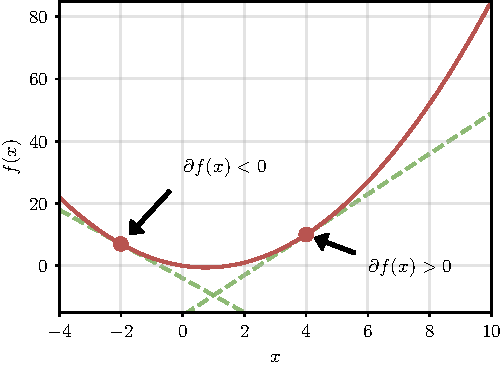
\includegraphics[width=0.6\textwidth]{images/gradient_info.pdf}
    \caption{График функции $f(x)=x^2 -1.5x$, показанный вместе с производными в двух разных точках.}
    \label{fig:derivative}
\end{SCfigure}


Мы напомним некоторые важные свойства производных, которые распространяются на многомерный случай:
%
\begin{itemize}
    \item \textbf{Линейность}: производная линейна, поэтому производная суммы равна сумме производных:
    %
    $$
    \partial \Big[{\color{drawred}f(x)} + {\color{drawgreen}g(x)}\Big] = {\color{drawred}{f}^\prime(x)} + {\color{drawgreen}g^\prime(x)} \,.
    $$
    \item \textbf{Правило произведения}:
    %
    $$
    \partial\Big[ {\color{drawred}f(x)}{\color{drawgreen}g(x)}\Big] = {\color{drawred}{f}^\prime(x)}{\color{drawgreen}g(x)} + {\color{drawred}f(x)}{\color{drawgreen}g'(x)} \,.
    $$
    \item \textbf{Цепное правило}: производная композиции функций задается умножением соответствующих производных:
    %
    \begin{equation}
        \partial \Big[{\color{drawred}f(}{\color{drawgreen}g(x)}{\color{drawred})}\Big] = {\color{drawred}{f^\prime}(}{\color{drawgreen}g(x)}{\color{drawred}}){ \color{drawgreen}g'(x)} \,
    \end{equation}
\end{itemize}

\subsection{Градиенты и производные по направлению}

Рассмотрим теперь функцию $y = f(\mathbf{x})$, принимающую на вход вектор $\mathbf{x} \sim(d)$. Говорить здесь о бесконечно малых возмущениях не имеет смысла, если мы не укажем направление этого возмущения (в то время как в скалярном случае у нас были только «влево» и «вправо», в этом случае у нас есть бесконечное количество возможных направлений в евклидовом пространстве). В простейшем случае мы можем рассмотреть движение вдоль $i$-й оси, сохраняя все остальные значения фиксированными:
%
\begin{equation}
\partial_{x_i} f(\mathbf{x}) = \frac{\partial y}{\partial x_i} = \lim_{h \rightarrow 0} \frac{f(\mathbf{x} + h\mathbf{e}_i) - f(\mathbf{x})}{h} \,.
\label{eq:partial_derivative}
\end{equation}
%
где $\mathbf{e}_i \sim (d)$ — это $i$-й базисный вектор ( $i$-я строка единичной матрицы):
%
\begin{equation}
\idx{\mathbf{e}_i}{j} = \begin{cases} 1 & \text{ если } i =j \\ 0 & \text{иначе} \end{cases}
\label{eq:basis_vector}
\end{equation}
%
\eqref{eq:partial_derivative} называется \textbf{частной производной}. Собирая все частные производные вместе, мы получаем $d$-мерный вектор, называемый \textbf{градиентом} функции.

\begin{definition}[Градиент] \addbottle
\textbf{Градиент} функции $y = f(\mathbf{x})$ задается как:
%
\begin{equation}
    \nabla f(\mathbf{x}) = \partial f(\mathbf{x})=\begin{bmatrix} \partial_{x_1} f(\mathbf{x}) \\ \vdots \\ \partial_{x_d} f(\mathbf{x}) \end{bmatrix}
\end{equation}
\end{definition}

Поскольку градиенты являются фундаментальными, мы используем специальное обозначение $\nabla f(\mathbf{x})$ для их выделения. А как насчет смещений в общем направлении $\mathbf{v}$? В этом случае мы получаем \textbf{производную по направлению}:
%
\begin{equation}
\mathrm{D}_{\mathbf{v}}f(\mathbf{x}) = \lim_{h \rightarrow 0} \frac{f(\mathbf{x} + h\mathbf{v}) - f(\mathbf{x})}{h} \,.
\label{eq:directional_derivative}
\end{equation}
%
Движение в пространстве можно разложить, рассматривая отдельные смещения вдоль каждой оси, поэтому легко доказать, что производная по направлению задается скалярным произведением градиента на вектор смещения $\mathbf{v}$:
%
\begin{equation}
\mathrm{D}_\mathbf{v} f(\mathbf{x})=\langle\nabla f(\mathbf{x}),\mathbf{v}\rangle = \sum_i \eqnmarkbox[drawred]{node}{\partial_{x_i} f(\mathbf{x})v_i}
\label{eq:directional_derivative_dot_product}
\end{equation}
\annotate[yshift=-1em]{below,right}{node}{Смещение по $i$-й оси}

Следовательно, умения вычислять градиент функции достаточно для вычисления всех возможных производных по направлению.

\subsection{Якобианы}

Рассмотрим теперь общий случай функции $\mathbf{y} = f(\mathbf{x})$ \addclock с векторным входом $\mathbf{x} \sim (d)$, как и раньше, и на этот раз с \textit{векторным} выходом $\mathbf{y} \sim(o)$. Как мы увидим, это самый общий случай, который нам нужно рассмотреть. Поскольку у нас более одного выхода, мы можем вычислить градиент для каждого выхода, и их стек дает матрицу $(o, d)$, которую мы называем \textbf{Якобианом} $f$.

\begin{definition}[Якобиан]
\textbf{Матрица Якоби} функции $\mathbf{y} = f(\mathbf{x})$, $\mathbf{x} \sim (d)$, $\mathbf{y} \sim (o)$ задается как:
%
\begin{equation}
\partial f(\mathbf{x}) = \begin{pmatrix}		\frac{\partial y_1}{\partial x_1} & \dots & \frac{\partial y_1}{\partial x_d} \\		\vdots & \ddots & \vdots \\		\frac{\partial y_o}{\partial x_1} & \dots & \frac{\partial y_o}{\partial x_d} \\	\end{pmatrix} \sim (o,d)
\end{equation}
\end{definition}

Мы получаем градиент при $o=1$ и стандартную производную при $d=o=1$. Якобианы наследуют все свойства производных: важно, что Якобиан композиции функций теперь является \textit{умножением матриц} соответствующих индивидуальных Якобианов:
%
\begin{equation}
\partial\left[f(g(\mathbf{x}))\right] = \left[\partial f(\bullet)\right]\partial g(\mathbf{x})
\label{eq:jacobian_chain_rule}
\end{equation}
%
где первая производная вычисляется в $g(\mathbf{x}) \sim (h)$. См. \cite[Глава 2]{petersen2008matrix} для численных примеров вычисленных градиентов и Якобианов. Как и в скалярном случае, градиенты и Якобианы можно понимать как линейные функции, касательные к определенной точке. В частности, градиент является наилучшим «приближением первого порядка» в следующем смысле. Для точки $\mathbf{x}_0$ наилучшее линейное приближение в бесконечно малой окрестности $f(\mathbf{x}_0)$ задается:

\vspace{0.5em}
$$
\widetilde{f}(\mathbf{x})= f(\mathbf{x}_0)+\langle \eqnmarkbox[drawred]{node}{\partial f(\mathbf{x}_0)}, \eqnmarkbox[drawgreen]{node2}{\mathbf{x}-\mathbf{x}_0} \rangle
$$
\annotate[yshift=1em]{above,right}{node}{Наклон прямой}
\annotate[yshift=-1em]{below,right}{node2}{Смещение от $\mathbf{x}_0$}

\vspace{0.5em}
Это называется \textbf{теоремой Тейлора}. См. Листинг \ref{code:taylor_approximation} и Рисунок \ref{fig:taylor_approximation} для визуализации в скалярном случае $f(x) = x^2 - 1.5x$.

\begin{mypy}{Пример вычисления приближения первого порядка (скалярный случай). Результат показан на Рисунке \ref{fig:taylor_approximation}.}{code:taylor_approximation}
# Общая функция
f = lambda x: x**2-1.5*x

# Производная (пока вычисляется вручную)
df = lambda x: 2*x-1.5 

# Линеаризация в точке 0.5
x=0.5
f_linearized = lambda h: f(x) + df(x)*(h-x) 

# Сравнение приближения с реальной производной
print(f(x + 0.01))            # [Out]: -0.5049
print(f_linearized(x + 0.01)) # [Out]: -0.5050
\end{mypy}

\begin{SCfigure}
    \centering
    \hspace{1em}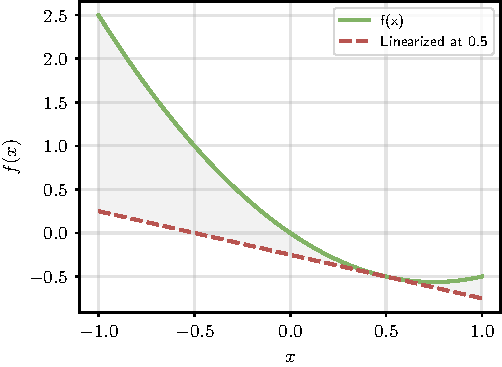
\includegraphics[width=0.6\textwidth]{images/taylor_approximation.pdf}
    \caption{Функция $f(x)=x^2-1.5x$ и ее приближение первого порядка, показанное в точке $0.5$.}
    \label{fig:taylor_approximation}
\end{SCfigure}

\subsection*{О размерности Якобианов \addteacup}
%
В заключение сделаем педантичное замечание о размерности, которое будет полезно в дальнейшем.   Рассмотрим следующую функцию:
%
$$
\mathbf{y} = \mathbf{W}\mathbf{x}
$$
%
При рассмотрении как функции от $\mathbf{x}$, производная, как и прежде, является матрицей $(o, d)$, и можно показать, что:
%
$$
\partial_{\mathbf{x}}\left[\mathbf{W}\mathbf{x}\right] =\mathbf{W}
$$
%
При рассмотрении как функции от $\mathbf{W}$, вход сам является матрицей $(o, d)$, и «Якобиан» в этом случае имеет форму $(o,o,d)$ (см. вставку на следующей странице). Однако мы всегда можем представить себе идентичную (изоморфную) функцию, принимающую на вход векторизованную версию $\mathbf{W}$, $\text{vect}(\mathbf{W})  \sim(od)$, и в этом случае Якобиан будет матрицей формы $(o, od)$.

Этот краткий пример проясняет, что мы имеем в виду под нашим утверждением, что работа с векторными входами и выходами «достаточна» с точки зрения нотации. Однако важно помнить об этом в Главе \ref{chap:automatic_differentiation}, когда мы будем использовать матричные Якобианы для простоты нотации (в частности, чтобы избежать размножения индексов), но размеры этих Якобианов могут «скрываться» внутри фактических форм входов и выходов, в первую очередь размеров пакетов. Важно отметить, что в Главе \ref{chap:automatic_differentiation} мы увидим, что явного вычисления Якобианов можно избежать на практике, рассматривая так называемые \textbf{векторно-якобианские произведения}. Это также можно формализовать, рассматривая Якобианы как абстрактные линейные отображения - см. \cite{blondel2024elements} для формального обзора этой темы.

\begin{supportbox}{Вычисление Якобиана}
Чтобы вычислить Якобиан $\partial_{\mathbf{W}} \mathbf{W}\mathbf{x}$, мы можем переписать выражение поэлементно как:
%
$$
y_i=\sum_j W_{ij}x_j
$$
%
откуда мы немедленно находим, что:
%
\begin{equation}
\frac{\partial y_i}{\partial W_{ij}}=x_j
\label{eq:partial_yi_wij}
\end{equation}
%
Обратите внимание, что для явной материализации Якобиана (хранения его в памяти) нам потребовалось бы много повторяющихся значений. Как мы увидим в Главе \ref{chap:automatic_differentiation}, этого можно избежать, потому что на практике нас интересует только применение Якобиана к другому тензору.
\label{supportbox:jacobian}
\end{supportbox}

\section{Численная оптимизация и градиентный спуск} 

\addclock Чтобы понять полезность доступа к градиентам, рассмотрим задачу минимизации общей функции $f(\mathbf{x})$, где $\mathbf{x} \sim (d)$: 
%
\begin{equation}
\mathbf{x}^* = \underset{\mathbf{x}}{\arg\min} \; f(\mathbf{x})
\label{eq:optimization}
\end{equation}
%
где, аналогично $\argmax$, $\arg\min \; f(\mathbf{x})$ обозначает операцию нахождения значения $\mathbf{x}$, соответствующего наименьшему возможному значению $f(\mathbf{x})$. Мы предполагаем, что функция имеет один выход (\textbf{однокритериальная оптимизация}), и что область, по которой мы оптимизируем $\mathbf{x}$, не ограничена. 

В остальной части книги $\mathbf{x}$ будет кодировать параметры нашей модели, а $f$ будет описывать производительность самой модели на наших данных, что называется \textbf{обучением с учителем}, которое мы вводим в следующей главе. Мы можем рассматривать минимизацию вместо максимизации без потери общности, поскольку минимизация $f(\mathbf{x})$ эквивалентна максимизации $-f(\mathbf{x})$ и наоборот (чтобы это представить, подумайте о функции в 1D и поверните ее вокруг оси $x$, представляя, что происходит с ее низкими точками).

В очень редких случаях мы можем выразить решение в замкнутой форме (мы увидим один пример в контексте оптимизации методом наименьших квадратов в Разделе \ref{subsec:least_squares}). Однако в общем случае мы вынуждены прибегать к итерационным процедурам. Предположим, мы начинаем со случайного предположения $\mathbf{x}_0$ и на каждой итерации делаем шаг, который мы раскладываем на его величину $\eta_t$ (длину шага) и направление $\mathbf{p}_t$:

\vspace{1em}
\begin{equation}
\mathbf{x}_t = \eqnmarkbox[drawred]{node}{\mathbf{x}_{t-1}} + \eqnmarkbox[drawblue]{node2}{\eta_t\mathbf{p}_t}
\label{eq:iterative_descent}
\end{equation}
\annotate[yshift=1em]{above,right}{node}{Предположение на итерации $t$}
\annotate[yshift=-1em]{below,right}{node2}{Смещение на итерации $t$}

\vspace{1em}
Мы называем $\eta_t$ \textbf{размером шага} (или, в терминологии машинного обучения, \textbf{скоростью обучения}, по причинам, которые станут ясны в следующей главе). Направление $\mathbf{p}_t$, для которого существует $\eta_t$ такое, что $f(\mathbf{x}_t) \le f(\mathbf{x}_{t-1})$, называется \textbf{направлением спуска}. Если мы можем выбирать направление спуска на каждой итерации, и если мы осторожны в выборе размера шага, итерационный алгоритм в \eqref{eq:iterative_descent} сойдется к минимуму в смысле, который будет описан в ближайшее время.

Для дифференцируемых функций мы можем точно определить все направления спуска, используя производную по направлению из \eqref{eq:directional_derivative}, поскольку их можно определить как направления, вызывающие отрицательное изменение по отношению к нашему предыдущему предположению $\mathbf{x}_{t-1}$:
%
$$
\mathbf{p}_t \text{ является направлением спуска} \;\;\Rightarrow\;\; \mathrm{D}_{\mathbf{p}_t} f(\mathbf{x}_{t-1}) \le 0
$$
%
Используя то, что мы узнали в Разделе \ref{sec:gradients_and_jacobians}, и определение скалярного произведения через косинусное сходство из \eqref{eq:dot_product_cosine}, мы получаем:
%
$$
\mathrm{D}_{\mathbf{p}_t} f(\mathbf{x}_{t-1})=\langle \nabla f(\mathbf{x}_{t-1}), \mathbf{p}_t\rangle=\lVert\nabla f(\mathbf{x}_{t-1})\rVert \lVert\mathbf{p}_t\rVert \cos(\alpha)
$$
%
где $\alpha$ — угол между $\mathbf{p}_t$ и $\nabla f(\mathbf{x}_{t-1})$. Рассматривая выражение справа, первый член является константой по отношению к $\mathbf{p}_t$. Поскольку мы предположили, что $\mathbf{p}_t$ кодирует только направление движения, мы также можем безопасно ограничить его до $\lVert\mathbf{p}_t\rVert = 1$, делая второй член еще одной константой. Следовательно, по свойствам косинуса мы заключаем, что любое $\mathbf{p}_t$, чей угол с $\nabla f(\mathbf{x}_{t-1})$ находится между $\pi/2$ и $3\pi/2$, является направлением спуска. Среди них направление $\mathbf{p}_t = -\nabla f(\mathbf{x}_{t-1})$ (с углом $\pi$) имеет наименьшую возможную производную по направлению, и мы называем его \textbf{направлением наискорейшего спуска}. 

Соединив это понимание с итерационной процедурой в \eqref{eq:iterative_descent}, мы получаем алгоритм для минимизации любой дифференцируемой функции, который мы называем \textbf{(наискорейшим) градиентным спуском}.

\begin{definition}[(Наискорейший) Градиентный спуск] \addbottle
Для дифференцируемой функции $f(\mathbf{x})$, начальной точки $\mathbf{x}_0$ и последовательности размеров шага $\eta_t$, \textbf{градиентный спуск} выполняется как:
%
\begin{equation}
\mathbf{x}_{t}=\mathbf{x}_{t-1}-\eta_t\nabla f(\mathbf{x}_{t-1})
\label{eq:gradient_descent}
\end{equation}
\end{definition}

Мы не будем заниматься проблемой поиска подходящего размера шага, который мы просто будем считать «достаточно малым», чтобы итерация градиентного спуска обеспечивала уменьшение $f$. В следующем разделе мы сосредоточимся на том, какие точки получаются при запуске градиентного спуска из общей инициализации. Обратите внимание, что градиентный спуск так же эффективен, как и процедура, которую мы используем для вычисления градиента: мы представим общий эффективный алгоритм для этой цели в Главе \ref{chap:automatic_differentiation}.

\subsection{Сходимость градиентного спуска}

При обсуждении сходимости градиентного спуска нам нужно уточнить, что мы имеем в виду под «минимизатором» функции. Если вас не волнует сходимость и вы доверяете градиентному спуску, смело переходите к следующему разделу.

\begin{definition}[Минимум]
\textbf{Локальный минимум} $f(\mathbf{x})$ — это точка $\mathbf{x}^+$, такая, что для некоторого $\varepsilon > 0$ верно следующее:
%
$$
f(\mathbf{x}^+)\le f(\mathbf{x}) \;\;\; \forall \mathbf{x} \; :\; \eqnmarkbox[drawred]{node}{\lVert \mathbf{x}-\mathbf{x}^+ \rVert <\varepsilon}
$$
\annotate[yshift=-1em]{below,left}{node}{Шар размера $\varepsilon$ с центром в $\mathbf{x}^+$}

\end{definition}

Словами, значение $f(\mathbf{x}^+$) является минимумом, если мы рассматриваем достаточно малую окрестность $\mathbf{x}^+$. Интуитивно, в такой точке наклон касательной будет равен $0$, а градиент везде в окрестности $\mathbf{x}^+$ будет указывать вверх. Мы можем формализовать первую идею с помощью концепции \textbf{стационарных точек}.

\begin{definition}[Стационарные точки]
    \textbf{Стационарная точка} $f(\mathbf{x})$ — это точка $\mathbf{x}^+$, такая, что $\nabla f(\mathbf{x}^+)=0$.
\end{definition}

Стационарные точки не ограничиваются минимумами: они могут быть максимумами (минимумами $-f(\mathbf{x})$) или \textbf{седловыми точками}, которые являются точками перегиба, где кривизна функции меняется (см. Рисунок \ref{fig:saddle_point} для примера). В общем, без каких-либо ограничений на $f$, можно доказать, что градиентный спуск сходится только к общей стационарной точке в зависимости от его инициализации.

\begin{SCfigure}
    \centering
    \hspace{1em}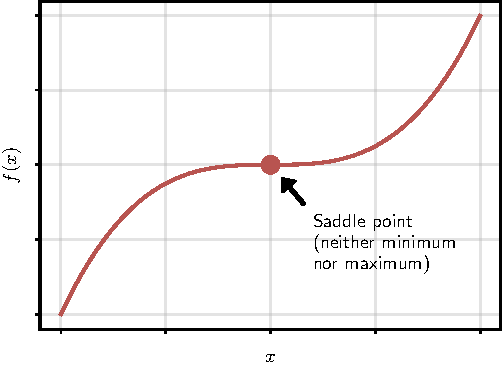
\includegraphics[width=0.6\textwidth]{images/saddle_point.pdf}
    \caption{Простой пример седловой точки (попробуйте представить касательную в этой точке, чтобы увидеть, что она действительно стационарна).}
    \label{fig:saddle_point}
\end{SCfigure}

Можем ли мы сделать лучше? Представьте себе параболу: в этом случае у функции нет седловых точек, и у нее есть только один минимум. Этот минимум также особенный, в том смысле, что функция в этой точке достигает своего наименьшего возможного значения во всей области определения: мы говорим, что это \textbf{глобальный минимум}.

\begin{definition}[Глобальный минимум]
    \textbf{Глобальный минимум} $f(\mathbf{x})$ — это точка $\mathbf{x}^*$, такая, что $f(\mathbf{x}^*) \le f(\mathbf{x})$ для любого возможного входа $\mathbf{x}$.
\end{definition}

Интуитивно, градиентный спуск сойдется к этому глобальному минимуму, если запустить его на параболе (из любой возможной инициализации), потому что все градиенты будут указывать на него. Мы можем обобщить эту идею с помощью концепции \textbf{выпуклости} функции. Существует много возможных определений выпуклости, мы выберем приведенное ниже для простоты изложения.

\begin{definition}[Выпуклая функция]
    Функция $f(\mathbf{x})$ является выпуклой, если для любых двух точек $\mathbf{x}_1$ и $\mathbf{x}_2$ и $\alpha \in \left[0,1\right]$ мы имеем:

    \vspace{1em}
    \begin{equation}
        f(\eqnmarkbox[drawblue]{node}{\alpha \mathbf{x}_1 + (1-\alpha)\mathbf{x}_2})\le \eqnmarkbox[drawred]{node2}{\alpha f(\mathbf{x}_1)+(1-\alpha)f(\mathbf{x}_2)}
        \label{eq:convex_function}
    \end{equation}
    \annotate[yshift=-1em]{below,right}{node}{Интервал от $\mathbf{x}_1$ до $\mathbf{x}_2$}
    \annotate[yshift=1em]{above,right}{node2}{Отрезок прямой от $f(\mathbf{x}_1)$ до $f(\mathbf{x}_2)$}
\end{definition}

\vspace{1em}
Левая часть в \eqref{eq:convex_function} — это значение $f$ в любой точке внутри интервала от $\mathbf{x}_1$ до $\mathbf{x}_2$, в то время как правая часть — это соответствующее значение на прямой, соединяющей $f(\mathbf{x}_1)$ и $f(\mathbf{x}_2)$. Если функция всегда находится ниже прямой, соединяющей любые две точки, она выпукла (например, парабола, направленная вверх, выпукла). 

Выпуклость характеризует простоту оптимизации функции в следующем смысле \cite{jain2017non}:
%
\begin{enumerate}
    \item Для общей \textit{невыпуклой} функции градиентный спуск сходится к \textit{стационарной точке}. Больше ничего нельзя сказать, если не смотреть на производные более высокого порядка (производные от производных).
    \item Для \textit{выпуклой} функции градиентный спуск сойдется к \textit{глобальному минимуму}, независимо от инициализации.
    \item  Если неравенство в \eqref{eq:convex_function} выполняется строго (\textbf{строгая выпуклость}), глобальный минимизатор также будет \textit{единственным}.
\end{enumerate}

Это жесткое свойство: чтобы найти глобальный минимум в невыпуклой задаче с помощью градиентного спуска, единственное решение — запускать оптимизатор бесконечное количество раз из всех возможных инициализаций, превращая это в NP-трудную задачу \cite{jain2017non}.

Это обсуждение имеет большое историческое значение. Как мы увидим в Главе \ref{chap:fully_connected_models}, любая нетривиальная модель является невыпуклой, что означает, что ее задача оптимизации может иметь несколько стационарных точек. Это контрастирует с альтернативными алгоритмами для обучения с учителем, такими как машины опорных векторов, которые сохраняют нелинейность, допуская при этом выпуклую оптимизацию. Интересно, что сложные дифференцируемые модели, кажется, хорошо работают даже перед лицом такого ограничения, в том смысле, что их оптимизация, при запуске из разумной инициализации, сходится к точкам с хорошей эмпирической производительностью.

\subsection{Ускорение градиентного спуска}
Отрицательный градиент описывает направление наискорейшего спуска, но только в бесконечно малой окрестности точки. Как мы увидим в Главе \ref{chap:deep_cnns} (где мы вводим стохастическую оптимизацию), эти направления могут быть чрезвычайно шумными, особенно при работе с большими моделями. Было разработано множество техник для ускорения сходимости алгоритма оптимизации путем выбора лучших направлений спуска. По вычислительным причинам нас особенно интересуют методы, которые не требуют производных более высокого порядка (например, Гессиана) или многократных вызовов функции.

Мы опишем здесь одну такую технику, \textbf{момент}, и отсылаем к \cite[Глава 12]{zhang2023dive} для более широкого введения.\footnote{См. также этот пост в блоге С. Рудера 2016 года: \url{https://www.ruder.io/optimizing-gradient-descent/}.} Если вы представляете градиентный спуск как шар, «катящийся с холма», движение относительно хаотично, потому что каждый градиент может указывать в совершенно другом направлении (фактически, при идеальном выборе размера шага и выпуклой функции потерь любые два градиента на последующих итерациях будут ортогональны). Мы можем сгладить это поведение, введя член «момента», который сохраняет некоторое направление от предыдущей итерации градиента:

\begin{align*}
\mathbf{g}_t& =- \eqnmarkbox[drawred]{node}{\eta_t\nabla f(\mathbf{x}_{t-1})} + \eqnmarkbox[drawblue]{node2}{\lambda\mathbf{g}_{t-1}} \\
\mathbf{x}_{t}& =\mathbf{x}_{t-1}+\mathbf{g}_t
\end{align*}
\annotate[yshift=1em]{above,right}{node}{Обычная итерация градиентного спуска}
\annotate[yshift=-1em]{below,right}{node2}{Дополнительный член момента}

где мы инициализируем $\mathbf{g}_0 = \mathbf{0}$. См. Рисунок \ref{fig:momentum} для примера. 

\begin{SCfigure}
    \centering
    \hspace{1em}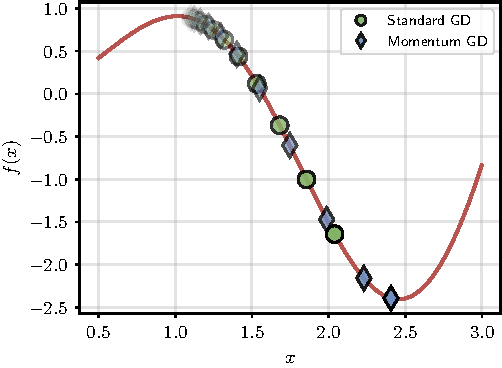
\includegraphics[width=0.6\textwidth]{images/momentum.pdf}
    \caption{Первые итерации стандартного GD и GD с моментом при минимизации $f(x)=x\sin(2x)$, начиная с $x=1+\varepsilon$, с $\lambda=0.3$.}
    \label{fig:momentum}
\end{SCfigure}

Коэффициент $\lambda$ определяет, насколько сильно затухает предыдущий член. Фактически, разворачивая два члена:
%
\begin{gather*}
\mathbf{g}_t=-\eta_t\nabla f(\mathbf{x}_{t-1}) +\lambda(-\eta_t\nabla f(\mathbf{x}_{t-2}) +\lambda\mathbf{g}_{t-2}) \\ = -\eta_t\nabla f(\mathbf{x}_{t-1}) -\lambda\eta_t\nabla f(\mathbf{x}_{t-2}) +\lambda^2\mathbf{g}_{t-2}
\end{gather*}
%
Обобщая, итерация в момент времени $t-n$ затухает с коэффициентом $\lambda^{n-1}$. Можно показать, что момент ускоряет обучение, сглаживая путь оптимизации \cite{sutskever2013importance}. Другой распространенной техникой является адаптация размера шага для каждого параметра на основе величины градиентов \cite{zhang2023dive}. Распространенным алгоритмом оптимизации, сочетающим несколько из этих идей, является Adam \cite{kingma2014adam}. Одним из преимуществ Adam является то, что он оказывается относительно устойчивым к выбору своих \textbf{гиперпараметров},\footnote{Гиперпараметр — это параметр, который выбирается пользователем, в отличие от того, который изучается градиентным спуском.} при этом выбор по умолчанию в большинстве фреймворков является хорошей отправной точкой в большинстве случаев.

Одним из недостатков использования ускоренных алгоритмов оптимизации могут быть увеличенные требования к хранению: например, момент требует, чтобы мы хранили предыдущую итерацию градиента в памяти, удваивая пространство, необходимое для алгоритма оптимизации (хотя в большинстве случаев, память, необходимая для вычисления градиента, является наиболее влиятельным фактором с точки зрения памяти, как мы увидим в Разделе \ref{sec:reverse_mode_automatic_differentiation}).

\newpage
\section*{От теории к практике}

\begin{supportbox}{Об упражнениях}
В этой книге нет классических упражнений в конце главы, которые рассматриваются во многих существующих учебниках. Вместо этого я описываю путь самообучения, чтобы помочь вам изучить два фреймворка (JAX и PyTorch) по мере продвижения по книге. Решения более практических упражнений будут опубликованы на веб-сайте книги.\footnote{\url{https://www.sscardapane.it/alice-book}} Эти разделы полны URL-ссылок на онлайн-материалы — они могут быть просрочены или перемещены к тому времени, как вы их будете искать.
\end{supportbox}

\subsection*{Начиная с основ: NumPy}

\begin{wrapfigure}{R}{3.0cm}
\vspace{-4em}
\includegraphics[width=3.0cm]{images/shutterstock_2075221579.jpg}
\vspace{-2em}
\end{wrapfigure} 

Отправной точкой для любого разработчика дифференцируемых моделей является тщательное изучение NumPy. NumPy реализует общий набор функций для манипулирования многомерными массивами (которые мы называем \textit{тензорами} в книге), а также функции для индексации и преобразования их содержимого. Вы можете прочитать больше в кратком руководстве по библиотеке.\footnote{\url{https://numpy.org/doc/stable/user/quickstart.html}} Вы должны чувствовать себя комфортно при работе с массивами в NumPy, особенно с их индексацией: репозиторий {\footnotesize\verb+rougier/numpy-100+}\footnote{\url{https://github.com/rougier/numpy-100}} предоставляет хорошую, медленную серию упражнений для проверки ваших знаний.

\subsection*{Переход к реалистичному фреймворку}

Несмотря на свое влияние, NumPy ограничен, в частности, в поддержке параллельного оборудования, такого как GPU (если не используются дополнительные библиотеки), и в отсутствии автоматического дифференцирования (введенного в Главе \ref{chap:automatic_differentiation}). JAX воспроизводит интерфейс NumPy, добавляя расширенную поддержку оборудования, автоматическое вычисление градиентов и дополнительные преобразования, такие как \textbf{векторизованное отображение} (\mintinline{python}{jax.vmap}). Фреймворки, такие как PyTorch, также реализуют NumPy-подобный интерфейс в своей основе, но они вносят незначительные коррективы в номенклатуру и функциональность и добавляют несколько высокоуровневых утилит для построения дифференцируемых моделей. Для целей этой главы вы можете бегло просмотреть документацию \mintinline{python}{jax.numpy.array} и \mintinline{python}{torch.tensor}, чтобы понять, насколько много у них общего с NumPy. Пока вы можете игнорировать высокоуровневые модули, такие как \mintinline{python}{torch.nn}. Мы еще поговорим о том, как спроектированы эти фреймворки, в Главе \ref{chap:automatic_differentiation}, после того как представим их механизм вычисления градиентов.

\subsection*{Реализация алгоритма градиентного спуска}

Чтобы освоиться со всеми тремя фреймворками (NumPy, JAX, PyTorch), я предлагаю повторить приведенное ниже упражнение трижды — каждый вариант должен занять всего несколько минут, если вы знаете синтаксис.  Рассмотрим 2D-функцию $f(\mathbf{x})$, $\mathbf{x} \sim (2)$, где мы принимаем область определения $[0,10]$:\footnote{Я попросил ChatGPT сгенерировать хорошую функцию с несколькими минимумами и максимумами. Больше ничего в книге не сгенерировано БЯМ, что, как мне кажется, становится важным уточнением.}
%
\begin{equation*}
    f(\mathbf{x}) = \sin(x_1) \cos(x_2) + \sin(0.5x_1) \cos(0.5x_2)
\end{equation*}
%
Прежде чем продолжить чтение книги, повторите это для каждого фреймворка:
%
\begin{enumerate}
\item Реализуйте функцию \textbf{векторизованным} способом, т.е. для матрицы $\mathbf{X} \sim (n,2)$ из $n$ входов она должна возвращать вектор $f(\mathbf{X}) \sim (n)$, где $\idx{f(\mathbf{X})}{i} = f(\mathbf{X}_i)$.
\item Реализуйте другую функцию для вычисления ее градиента (жестко закодированного — мы еще не касались автоматического дифференцирования).
\item Напишите базовую процедуру градиентного спуска и визуализируйте пути, пройденные процессом оптимизации из нескольких начальных точек.
\item Попробуйте добавить член момента и визуализировать норму градиентов, которая должна сходиться к нулю по мере движения алгоритма к стационарной точке.
\end{enumerate}
%
Если вы используете JAX или PyTorch для решения упражнения, пункт (3) — хорошее место для экспериментов с \mintinline{python}{vmap} для векторизации функции.